\section{Übersicht}

\begin{frame}
  {Übersicht}
  \onslide<+->
  \begin{itemize}[<+->]
    \item Wo stehen Kommata?
      \Zeile
    \item Doppelfunktion oder Monofunktion?
    \item Probleme
      \Zeile
    \item Empirie | \textit{obwohl} und \textit{weil} mit V2
      \Zeile
    \item \citet{Schaefer2018b,SchaeferSayatz2016}
  \end{itemize}
\end{frame}

\section[Befund]{Deskriptiver Befund}

\begin{frame}
  {Aufzählung}
  \onslide<+->
  \onslide<+->
  \begin{exe}
    \ex \alert{Peter, Paul und Mary} gehen in den Zoo.
    \ex \alert{Unter, neben und über} dem Werkstück für genügend Freiraum achten.
    \ex \alert{Wandern, Schwimmen, Radfahren} -- Volkssport pur!
    \ex Die Verbindung erfolgt \alert{form-, kraft- oder stoff}schlüssig.
  \end{exe}
  \onslide<+->
  \Zeile
  Kommatierung ist hier so flexibel wie Koordinationsstrukturen eben sind.
\end{frame}

\begin{frame}
  {Sätze}
  \onslide<+->
  \onslide<+->
  \begin{exe}
    \ex
    \begin{xlist}
	  \ex \grau{Die Sonne geht unter, der Mond geht auf.}
	  \ex \grau{Die Sonne geht unter, und der Mond geht auf.}
    \end{xlist}
    \Zeile
    \ex Adrianna weiß, \alert{dass es gleich regnen} \orongsch{wird}.
    \ex Michelle geht, \alert{obwohl die Party erst} \orongsch{beginnt}.
    \ex Adrianne hilft der Kollegin, \alert{die nassgeregnet} \orongsch{wurde}.
    \Zeile
    \ex \tuerkis{Adrianna glaubt, die Regenwolken zu sehen.}
  \end{exe}
  \onslide<+->
  \Zeile
  Diese Satzkommas lassen sich gut auf eine syntaktische Domäne eingrenzen.
\end{frame}

\begin{frame}
  {Sonstiges}
  \onslide<+->
  \onslide<+->
  \begin{exe}
    \ex Adrianna, \alert{eine Kollegin}, wurde nassgeregnet.
    \ex Die, \alert{übrigens unsinnige}, Behauptung der Monofunktion\\
    wird kaum vertreten.
    \ex Michelle will den Dobermann aufnehmen, \alert{als Pflegestelle}.
    \ex \alert{Ja}, Michelle kennt Adrianna.
  \end{exe}
  \onslide<+->
  \Zeile
  Hat das Komma hier primär einen Intonationseffekt?
\end{frame}

\section[Erklärung]{Erklärungsansätze}

\begin{frame}
  {Syntax | Doppelfunktion (Primus usw.)}
  \onslide<+->
  \onslide<+->
  Gibt es überhaupt eine "`Theorie des Kommas"'?\\
  \onslide<+->
  \Zeile
  \begin{itemize}[<+->]
    \item Nein | Ziel: \alert{optimale Beschreibungen von Verteilungen}\\
	    \Zeile
    \item syntaktisch keine Gemeinsamkeit zwischen Koordination und Nebensatz
    \item \ldots\ \alert{aber beides auf jeden Fall rein syntaktisch definierte Grenzen!}
	    \Halbzeile
    \item \alert{Intonationsgrenzen?} --- ja, als Folge der syntaktischen Grenze
    \item aber \rot{viele Intonationsgrenzen ohne Komma}
  \end{itemize}
\end{frame}


\begin{frame}
  {Syntax von Koordination}
  \alert{Verbindung von kategorial Gleichem zu kategorial Gleichem},\\
  kein Kopfstatus | beliebig simplexe oder komplexe Kategorien\\
  \Zeile
  \centering 
  \scalebox{0.8}{%
  \begin{forest}
    [\textbf{N}, calign=child, calign child=2
      [\textbf{N}, tier=preterminal
        [\it Kuchen]
      ]
      [Konj, tier=preterminal
        [{\it \alert{und}\ \slash\ \alert{,}}]
      ]
      [\textbf{N}, tier=preterminal
        [\it Sahne]
      ]
    ]
  \end{forest}}~\hspace{2em}~%
  \scalebox{0.8}{%
  \begin{forest}
    [S, calign=child, calign child=2
      [S, tier=preterminal
        [\it Es ist Sonntag, narroof]
      ]
      [Konj, tier=preterminal
        [{\it {und}\ \slash\ \alert{,}}]
      ]
      [S, tier=preterminal
        [\it die Zeit wird knapp, narroof]
      ]
    ]
  \end{forest}}
\end{frame}

\begin{frame}
  {Syntax von Satzeinbettung (Beispiel)}
  \alert{Strukturen mit (finitem) Verb und allen Abhängigen} |\\
  funktional Ergänzungen, Angaben, Attribute, evtl.\ max.\ eine Spur\\
  \Zeile
  \centering
  \scalebox{0.8}{%
  \begin{forest}
    [NP, calign=child, calign child=2
      [Art, tier=preterminal
        [\it einen]
      ]
      [\bf N, tier=preterminal
        [\it Tofu \alert{,}]
      ]
      [RS, calign=first
        [NP\Sub{1}, tier=preterminal
          [\it der, narroof, name=BeweDer]
        ]
        [VP, calign=last
          [NP, tier=preterminal
            [\it mir, narroof]
          ]
          [\Ti, tier=preterminal]
          {\draw[dotted, thick, ->] (.south) |- ++(0,-4.5em) -| (BeweDer.south);}
          [Ptkl, tier=preterminal
            [nicht]
          ]
          [\bf V, calign=last
            [\bf V, tier=preterminal
              [\it geschmeckt]
            ]
            [\bf V, tier=preterminal
              [\it hat]
            ]
          ]
        ]
      ]
    ]
  \end{forest}}
\end{frame}

\begin{frame}
  {Syntax | Bredels Monofunktion I}
  \onslide<+->
  \begin{itemize}[<+->]
	  \item Behauptung | \alert{Doppelfunktion "`nicht lernbar"'}
		  \Zeile
    \item Wie bitte?
	    \Halbzeile
	    \begin{itemize}[<+->]
		    \item \alert{Homonymie?}\\
			    \textit{Kiefer}, \textit{Schloss}, \textit{Bank}
			    \Halbzeile
		    \item \alert{Synkretismus?}\\
			    \textit{dieser}, \textit{Menschen}, \textit{laufen}
			    \Halbzeile
		    \item \alert{strukturelle Ambiguität?}\\
			    \textit{Scully beobachtet den Außerirdischen mit dem Teloskop.}
	    \end{itemize}
  \end{itemize}
\end{frame}

\begin{frame}
  {Syntax | Bredels Monofunktion II}
  \onslide<+->
  \begin{itemize}[<+->]
	  \item Komma markiert \alert{"`Grenze im Parsingprozess"'}
          \item kein normales Weiterparsen wie vorher
	  \item also "`Online-Funktion"' in der Syntaxverarbeitung
		  \Halbzeile
	  \item \rot{keine} zugrundeliegende Syntaxtheorie\\
            \grau{Es gibt formale Theorien inkrementeller Verarbeitung!}
	  \item \rot{keine} ausgearbeitete Verabreitungstheorie
            \Halbzeile
	  \item beliebig \rot{allgemeine Beschreibung} = immer Monofunktion\\
		  \grau{Die Funktion jedes Wortes ist die sprachliche Kommunikation!}
  \end{itemize}
\end{frame}

\begin{frame}
  {Syntax | Bredels Monofunktion III}
  \onslide<+->
  \onslide<+->
  Die (Fremd-)Daten sind nicht falsch, nur die Schlussfolgerung.\\
  \Zeile
  \begin{itemize}[<+->]
	  \item ähnlich wie bei der NP-Kopf-Großschreibung \ldots
            \Halbzeile
		  \begin{itemize}[<+->]
                          \item \alert{natürlich} markiert Komma irgendwelche Phrasengrenzen
			  \item \alert{natürlich} beim Parsen (Verarbeitung) wichtiges Indiz
				  \Halbzeile
			  \item \grau{Das steht bei den Psycholinguisten, die Bredel rezipiert.}
				  \Halbzeile
			  \item \rot{Aber das erklärt nicht die Verteilung von Kommata im Deutschen!}
		  \end{itemize}
  \end{itemize}
\end{frame}

\begin{frame}
  {Probleme | Satzverbindungen}
  \onslide<+->
  \onslide<+->
  "`Vor \textit{und} steht kein Komma."'\\
  \Zeile
  \onslide<+->
  \begin{exe}
    \ex[ ]{Die Sonne geht unter\alert{,} der Mond geht auf.}
    \ex[ ]{Die Sonne geht unter\alert{, und} der Mond geht auf.}
    \ex[?]{Die Sonne geht unter\rot{, und} die Schlacht von Worringen fand 1288 statt.}
  \end{exe}
  \Zeile
  \begin{itemize}[<+->]
    \item Konflikt | Aufzählungskomma (nie mit \textit{und}) und Satzkomma
    \item Bedingung für Satzkomma stärker \ding{220} \rot{kein Aufzählungskomma}
    \item außerdem spezielle semantische\slash pragmatische Bedingungen\\
      für Verknüpfung, also keine einfache Aufzählung
  \end{itemize}
\end{frame}

\begin{frame}
  {Probleme | Adversative Koordinationspartikeln}
  \onslide<+->
  \onslide<+->
  Warum steht hier ein Komma?\\
  \onslide<+->
  \Zeile
  \begin{exe}
    \ex
    \begin{xlist}
      \ex Wir fahren ein blaues \alert{und} elegantes Auto.
      \ex In der Küche \alert{und} in der Kammer stehen Wäschekörbe.
    \end{xlist}
    \ex
    \begin{xlist}
      \ex Wir fahren ein blaues\rot{, aber} elegantes Auto.
      \ex Nicht in der Küche\rot{, sondern} in der Kammer steht der Wäschekorb.
    \end{xlist}
  \end{exe}
  \Zeile
  \begin{itemize}[<+->]
    \item meines Erachtens nicht systemkonform
    \item \rot{semantisch\slash pragmatisch} motivierte Regel
    \item atypisch für das Deutsche
  \end{itemize}
\end{frame}

\begin{frame}
  {Probleme | \textit{Infinitvkonstruktionen}}
  \begin{exe}
    \ex[*]{Nadezhda \rot{scheint}, die Kontrolle über die Hantel zu verlieren.}
    \ex[*]{Nadezhda \rot{will}, die Weltmeisterschaft gewinnen.}
    \ex[ ]{Nadezhda \alert{beschließt}, keine Steroide mehr einzunehmen.}
    \ex[?]{Nadezhda \alert{beschließt}\orongsch{,} zu trainieren.}
  \end{exe}
  \onslide<+->
  \Zeile
  \begin{itemize}[<+->]
    \item \alert{Infinitivsyntax} ist der Schlüssel
    \item Komma nur bei \alert{inkohärenten Infinitiven}
  \end{itemize}
\end{frame}

\begin{frame}
  {Probleme | Inkohärente Infinitive}
  Kohärente und inkohärente Infinitivkonstruktionen\\
  \onslide<+->
  \Zeile
  \centering
  \scalebox{0.7}{%
  \begin{forest}
    [VP\Sub{1+2}, calign=last
      [NP, tier=preterminal
        [\textit{Vanessa}, narroof]
      ]
      [NP, tier=preterminal
        [\textit{die Pferde}, narroof]
      ]
      [\textbf{V\Sub{2+1}}, calign=last
        [\textbf{V\Sub{2}}, tier=preterminal
          [\textit{behufen}]
        ]
        [\textbf{V\Sub{1}}, tier=preterminal
          [\textit{will}]
        ]
      ]
    ]
  \end{forest}}~\hspace{2em}~%
  \scalebox{0.7}{%
  \begin{forest}
    l sep+=3em, s sep+=2em
    [VP\Sub{1}, calign=last
      [NP, tier=preterminal
        [\textit{Vanessa}, narroof]
      ]
      [VP\Sub{2}, calign=last
        [NP, tier=preterminal
          [\textit{die Pferde}, narroof]
        ]
        [\textbf{V\Sub{2}}, tier=preterminal
          [\textit{zu behufen}]
        ]
      ]
      [\textbf{V\Sub{1}}, tier=preterminal
        [\textit{wünscht}]
      ]
    ]
  \end{forest}}
\end{frame}

\begin{frame}
  {Probleme | Inkohärente Infinitve}
  \onslide<+->
  \onslide<+->
    \resizebox{1\textwidth}{!}{
    \begin{tabular}{lcllll}
      \lsptoprule
      & \multirow{2}{*}{\textbf{Status}} & \multirow{2}{*}{\textbf{Kohärenz}} & \textbf{eigenes} & \textbf{Subjekts-} \\
      & & & \textbf{Subjekt} & \textbf{Rolle} & \textbf{Beispiel}\\
      \midrule
      \textbf{Modalverben} & 1 & obl.\ kohärent & ja & Identität & \textit{wollen} \\
      \textbf{Halbmodalverben} & 2 & obl.\ kohärent & nein & nein & \textit{scheinen} \\
      \textbf{Kontrollverben} & 2 & \rot{opt.\ inkohärent} & ja & Kontrolle & \textit{beschließen} \\
      \lspbottomrule
    \end{tabular}
  }\\
  \Zeile
  \begin{itemize}[<+->]
    \item Nur \alert{inkohärente nachgestellte Infinitive} werden kommatiert!
    \item Sie gelten als satzwertig, aber \rot{Inkohärenz leider nur optional}.
    \item Es kommen also nur \alert{Abhängige von Halbmodalen} infrage.
  \end{itemize}
  \onslide<+->
  \Viertelzeile
  \begin{exe}
    \ex[*]{Nadezhda \rot{scheint}, die Kontrolle über die Hantel zu verlieren.}
    \ex[*]{Nedezhda \rot{will}, die Weltmeisterschaft gewinnen.}
  \end{exe}
\end{frame}

\begin{frame}
  {Probleme | Inkohärente Infinitve}
  \onslide<+->
  \onslide<+->
  Was ist jetzt hiermit?\\
  \Halbzeile
  \onslide<+->
  \begin{exe}
    \ex[ ]{Nadezhda \alert{beschließt}, keine Steroide mehr einzunehmen.}
    \ex[?]{Nadezhda \alert{beschließt}\orongsch{,} zu trainieren.}
  \end{exe}
  \onslide<+->
  \Halbzeile
  \alert{Eindeutig inkohärent} | hinter die RSK versetzte Infinitive\\
  \Viertelzeile
  \onslide<+->
  \begin{exe}
    \ex \rot{\textbf{Inkohärent}}
    \begin{xlist}
      \ex[ ]{\ldots dass Nadezhda beschließt, keine Steroide mehr zu nehmen.}
      \ex[*]{\ldots dass Nadezhda keine Steroide mehr zu nehmen beschließt.}
    \end{xlist}
    \ex \alert{\textbf{Kohärent oder inkohärent}}
    \begin{xlist}
      \ex[ ]{\ldots dass Nadezhda zu trainieren beschließt.}
      \ex[ ]{\ldots dass Nadezhda beschließt zu trainieren.}
    \end{xlist}
  \end{exe}
\end{frame}


\begin{frame}
  {Probleme | Inkohärente Infinitve}
  Es liegt also an der syntaktischen Struktur.\\
  \Zeile
  \onslide<+->
  \begin{exe}
    \ex
    \begin{xlist}
      \ex[ ]{[Nadezhda]\Sub{2} \alert{[beschließt]\Sub{1}} [t\Sub{2} \gruen{t\Sub{3}} \alert{[t\Sub{1}]\Sub{VK}}]\ \Sub{VP}\ \orongsch{,}\\
        {\hspace{1em}}\gruen{[keine Steroide mehr einzunehmen]\Sub{3}}.}
        \Viertelzeile
      \ex[*]{[Nadezhda]\Sub{2} \rot{[beschließt]\Sub{1}}\\
        {\hspace{1em}}[t\Sub{2} [keine Steroide] [mehr] \rot{[einzunehmen t\Sub{1}]\Sub{VK}}\ ]\Sub{VP}.}
    \end{xlist}
    \Halbzeile
    \ex
    \begin{xlist}
      \ex[ ]{[Nadezhda]\Sub{2} \alert{[beschließt]\Sub{1}}\ \orongsch{,} [t\Sub{2} \gruen{t\Sub{3}} \alert{[t\Sub{1}]\Sub{VK}}\ ]\Sub{VP} \gruen{[zu trainieren]\Sub{3}}.}
      \Viertelzeile
      \ex[ ]{[Nadezhda]\Sub{2} \tuerkis{[beschließt]\Sub{1}} [t\Sub{2} \tuerkis{[zu trainieren t\Sub{1}]\Sub{VK}}\ ]\Sub{VP}}
    \end{xlist}
  \end{exe}
  \Halbzeile
  \onslide<+->
  Füllen Sie den VK durch Hinzufügen von Hilfsverben auf,\\
  um das Phänomen noch deutlicher zu sehen.
\end{frame}

\begin{frame}
  {Probleme | Herausstellungen und Nichtintegration}
  \onslide<+->
  \onslide<+->
  \begin{exe}
    \ex Adrianna, \alert{eine Kollegin}, wurde nassgeregnet.
    \ex Die, \alert{übrigens unsinnige}, Behauptung der Monofunktion\\
    wird kaum vertreten.
    \ex Michelle will den Dobermann aufnehmen, \alert{als Pflegestelle}.
    \ex \alert{Ja}, Michelle kennt Adrianna.
  \end{exe}
  \onslide<+->
  \Halbzeile
  \begin{itemize}[<+->]
    \item \alert{Parenthesen} und \alert{Herausstellungen} im weiteren Sinn
    \item am ehesten Bredels Unterbrechung im Parsing
    \item bzw.\ \alert{Unterbrechung in der syntaktischen Struktur}
    \item die \alert{dritte Kommafunktion}?
      \Halbzeile
    \item Nanna Fuhrhop | "`pränominale Herausstellung ist Bindestrichfunktion"'\\
      \rot{entspricht aber nicht der Realität} (s.\ Sayatz und Schäfer i.\,V.)
  \end{itemize}
\end{frame}

\section[Empirie]{Funktion und Empirie | \citet{SchaeferSayatz2016}}

\begin{frame}
  {\textit{obwohl} und \textit{weil} mit V2}
  \centering 
  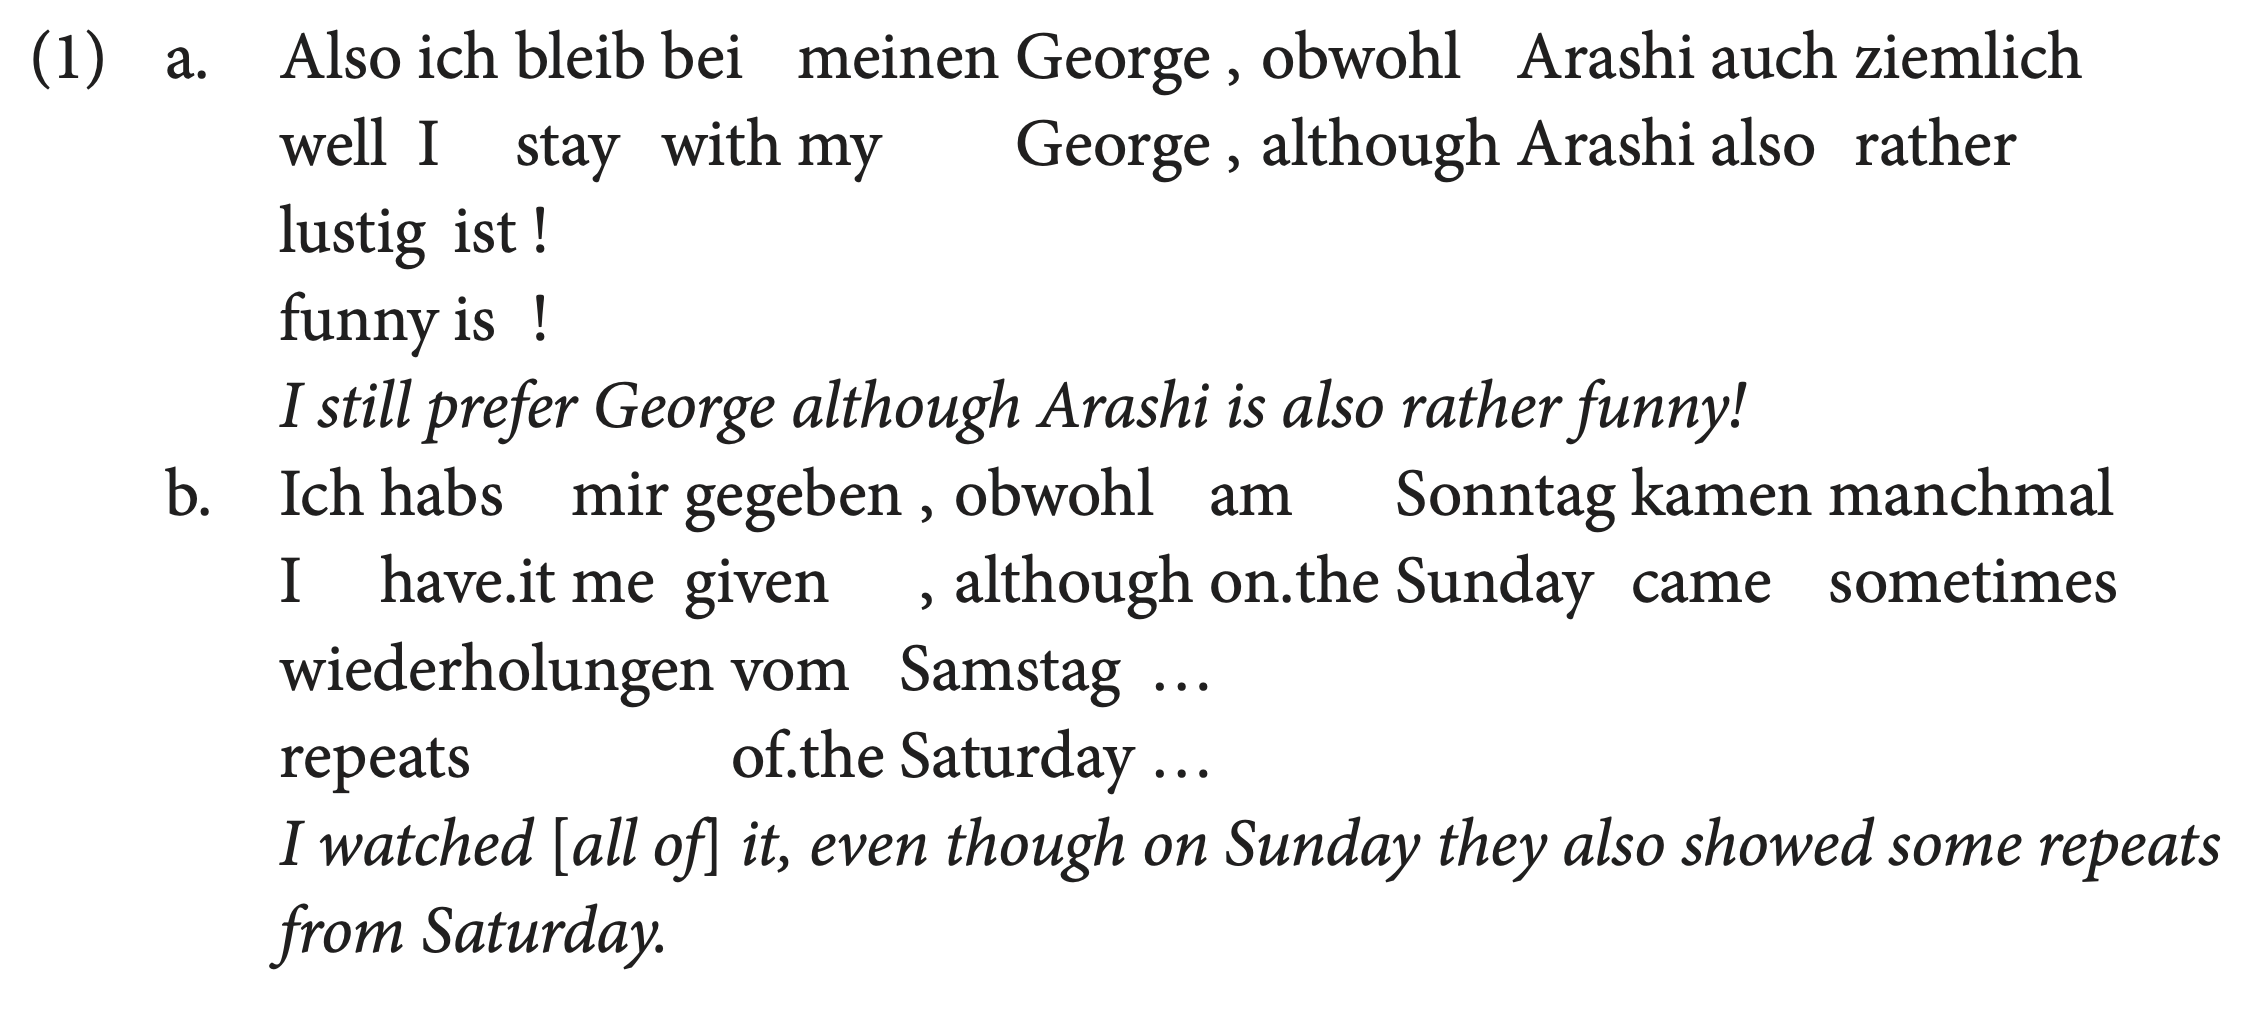
\includegraphics[width=0.7\textwidth]{\GRAPHPATH/obweil/01-obwohl}
\end{frame}

\begin{frame}
  {\textit{obwohl} und \textit{weil} mit V2}
  \centering 
  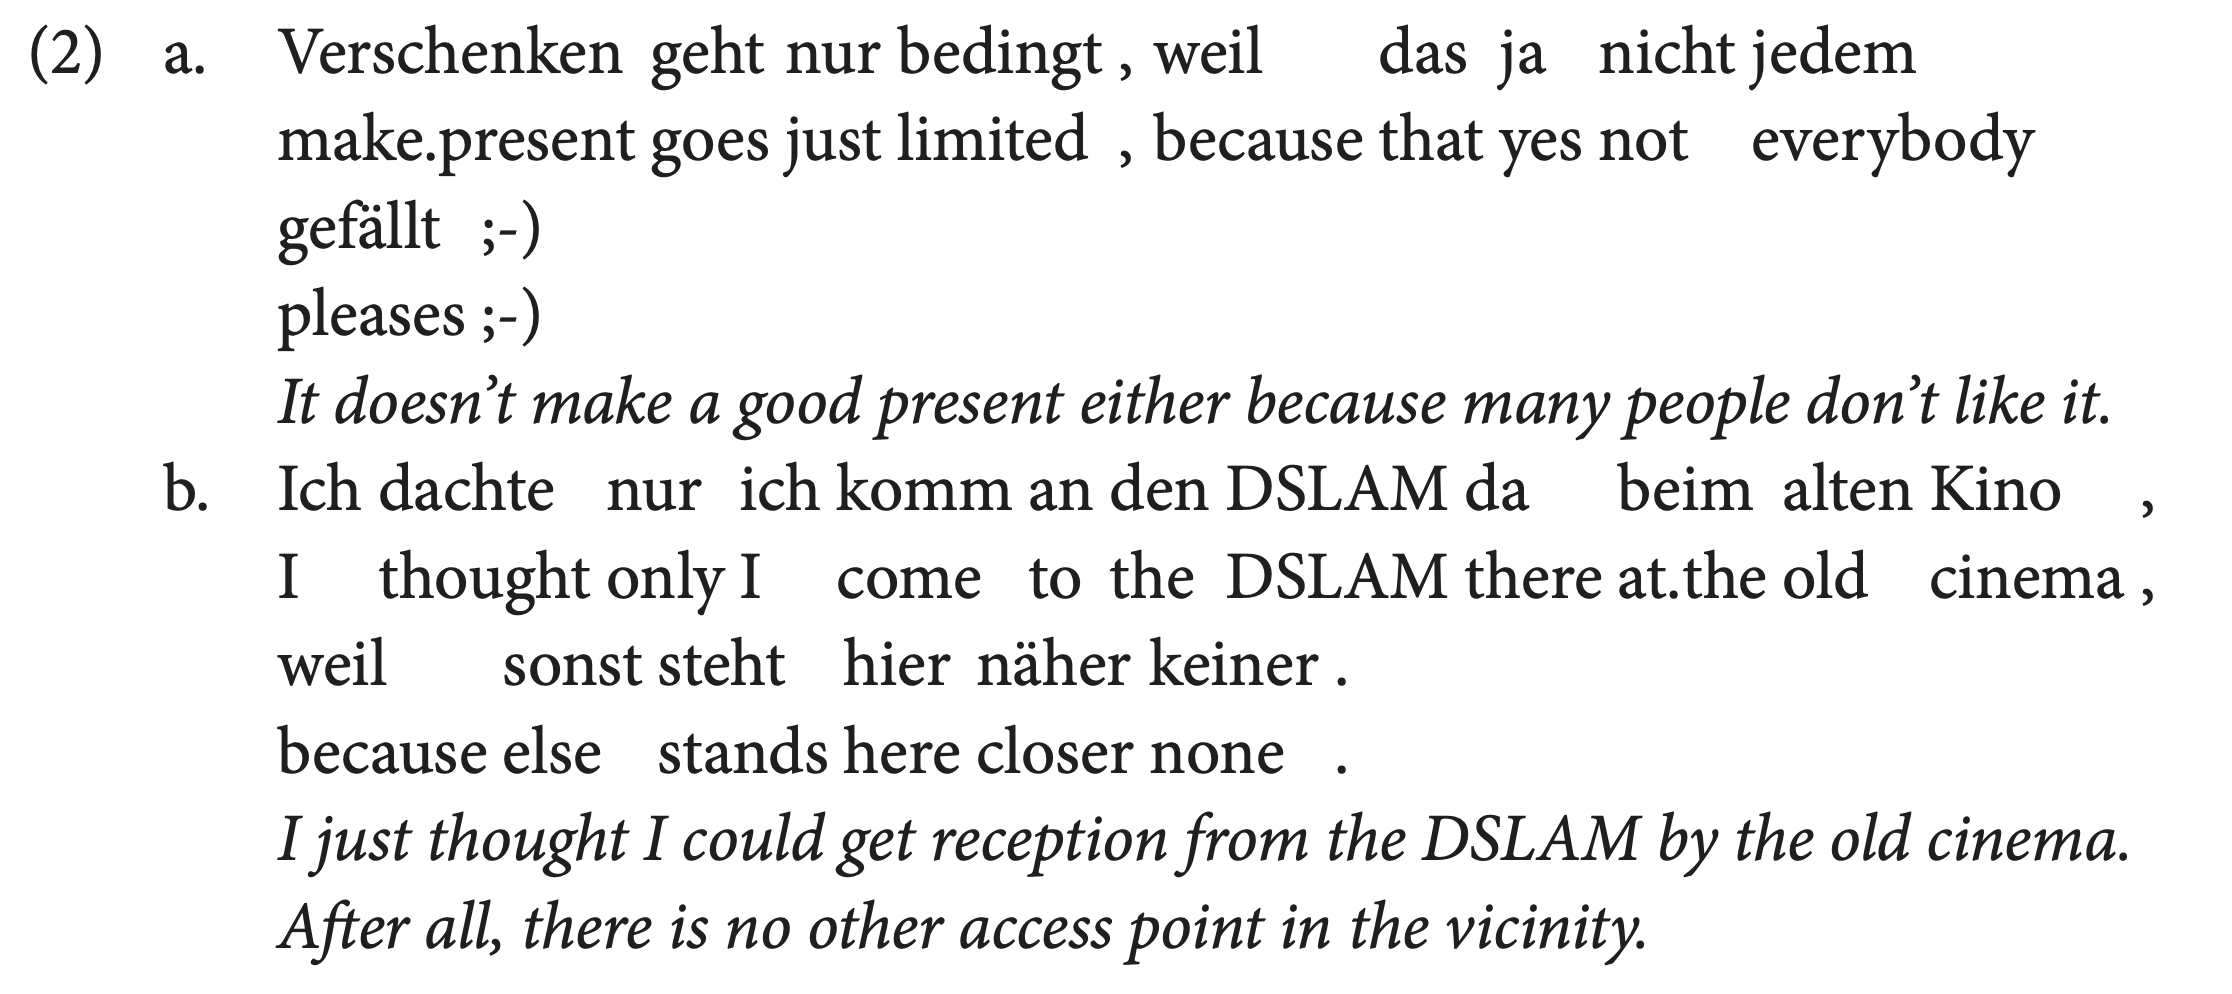
\includegraphics[width=0.7\textwidth]{\GRAPHPATH/obweil/01-weil}
\end{frame}

\begin{frame}
  {Variation der Interpunktion (Beispiele)}
  \centering 
  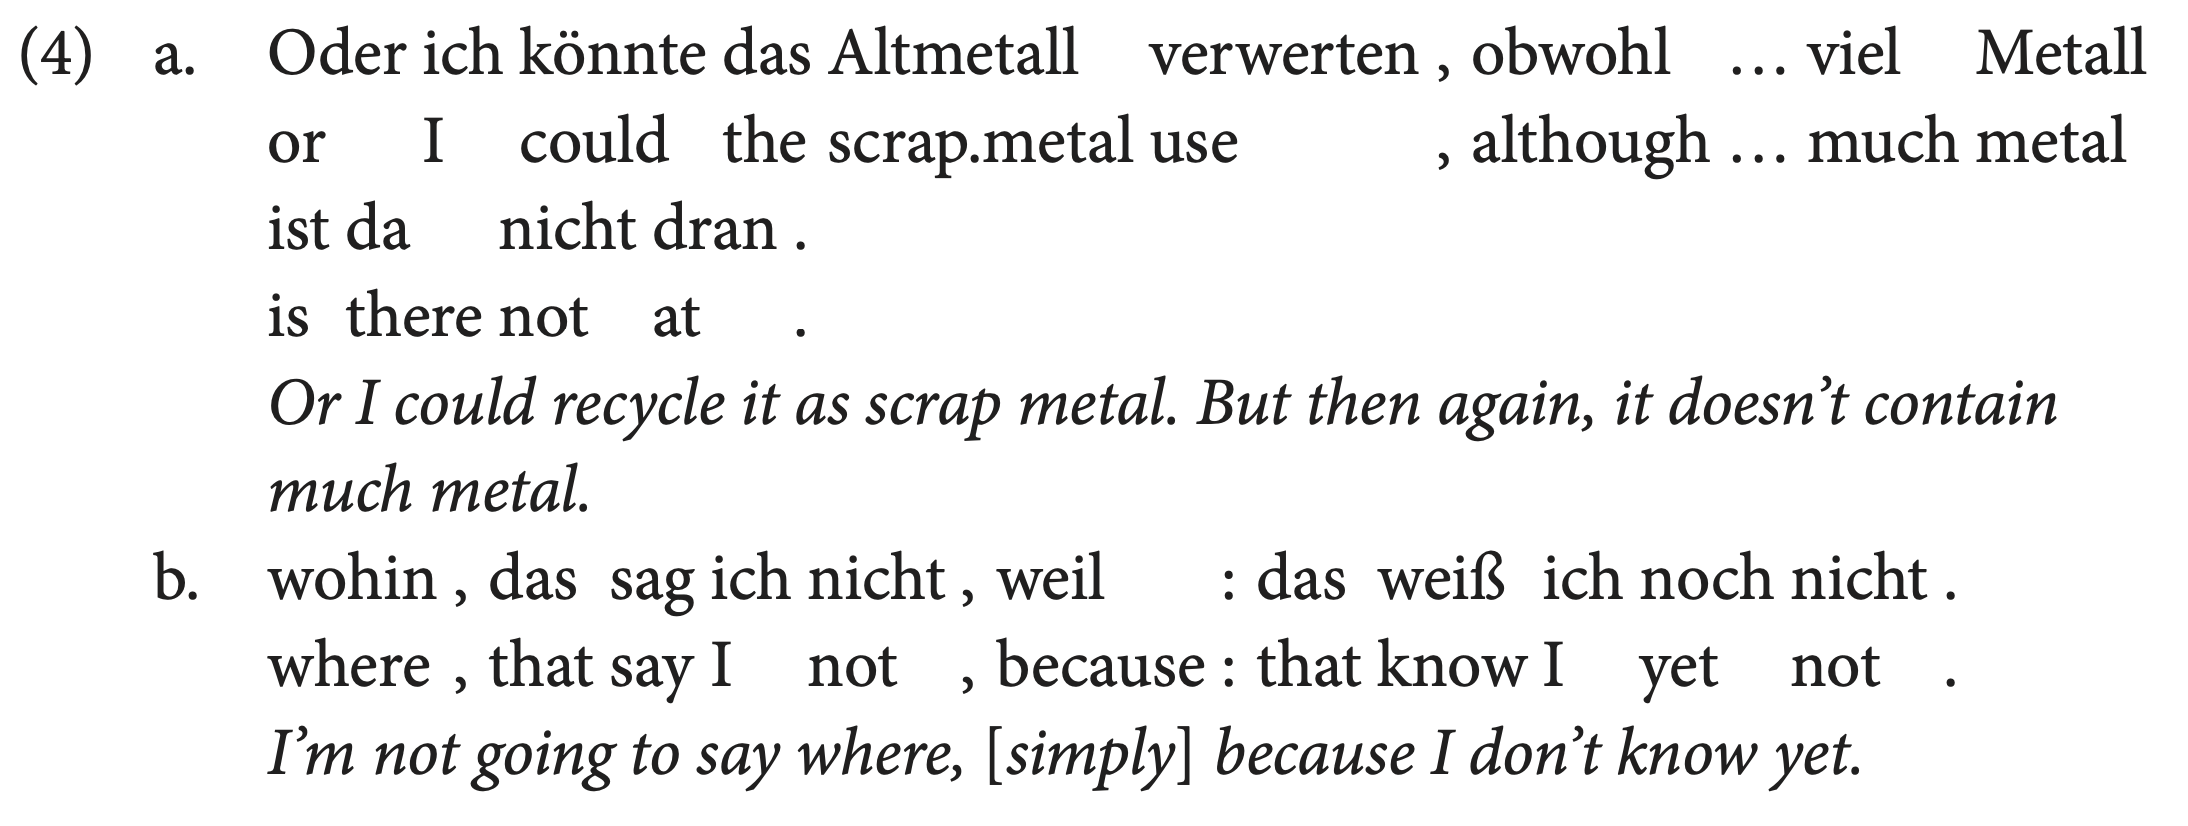
\includegraphics[width=0.7\textwidth]{\GRAPHPATH/obweil/02-interpunktion}
\end{frame}

\begin{frame}
  {Unabhängigkeit von Sätzen}
  \centering 
  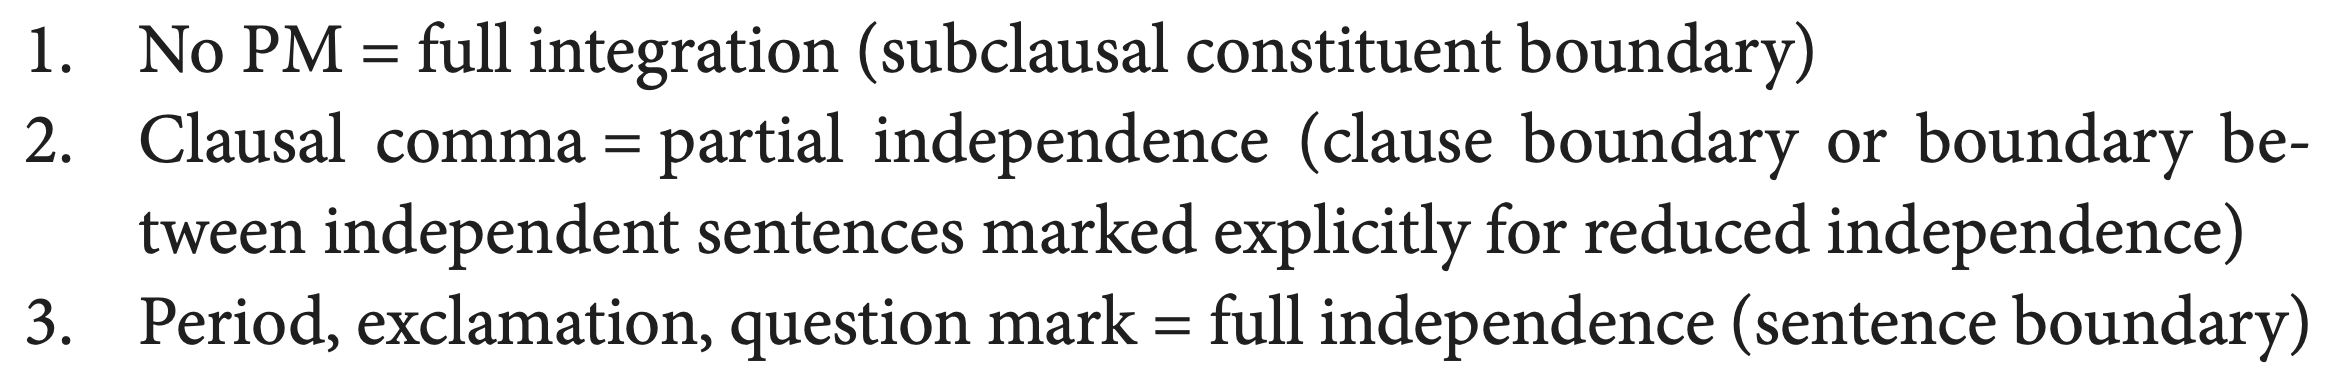
\includegraphics[width=0.7\textwidth]{\GRAPHPATH/obweil/03-independence} 
\end{frame}

\begin{frame}
  {Empirischer Befund I | Satzinitiale Partikeln}
  \centering 
  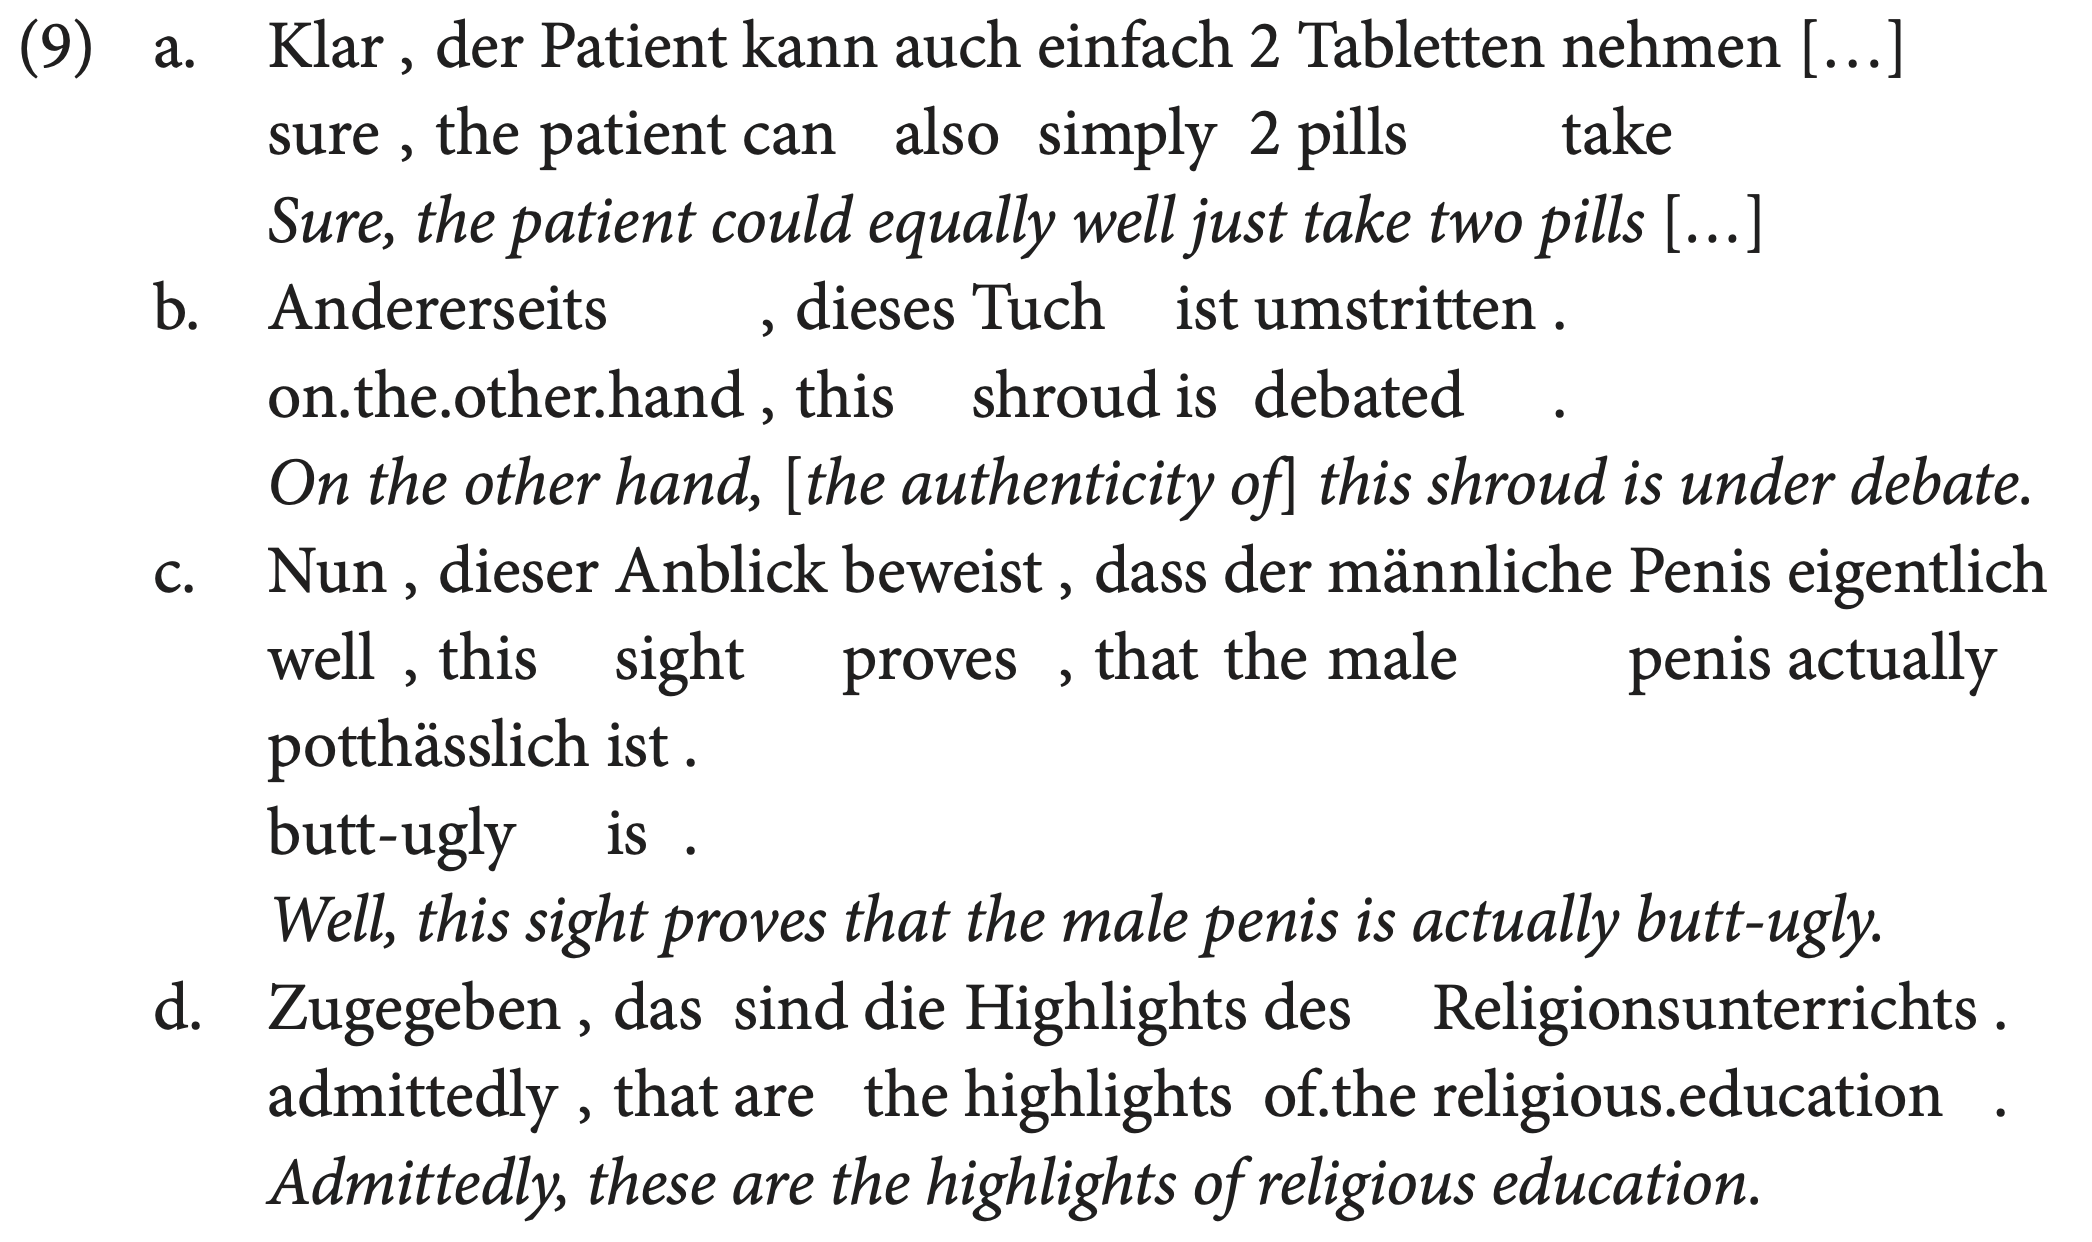
\includegraphics[width=0.7\textwidth]{\GRAPHPATH/obweil/04-satzinitial}
\end{frame}

\begin{frame}
  {Empirischer Befund II/1 | Wortverteilung bei Doppelpunkt}
  \centering 
  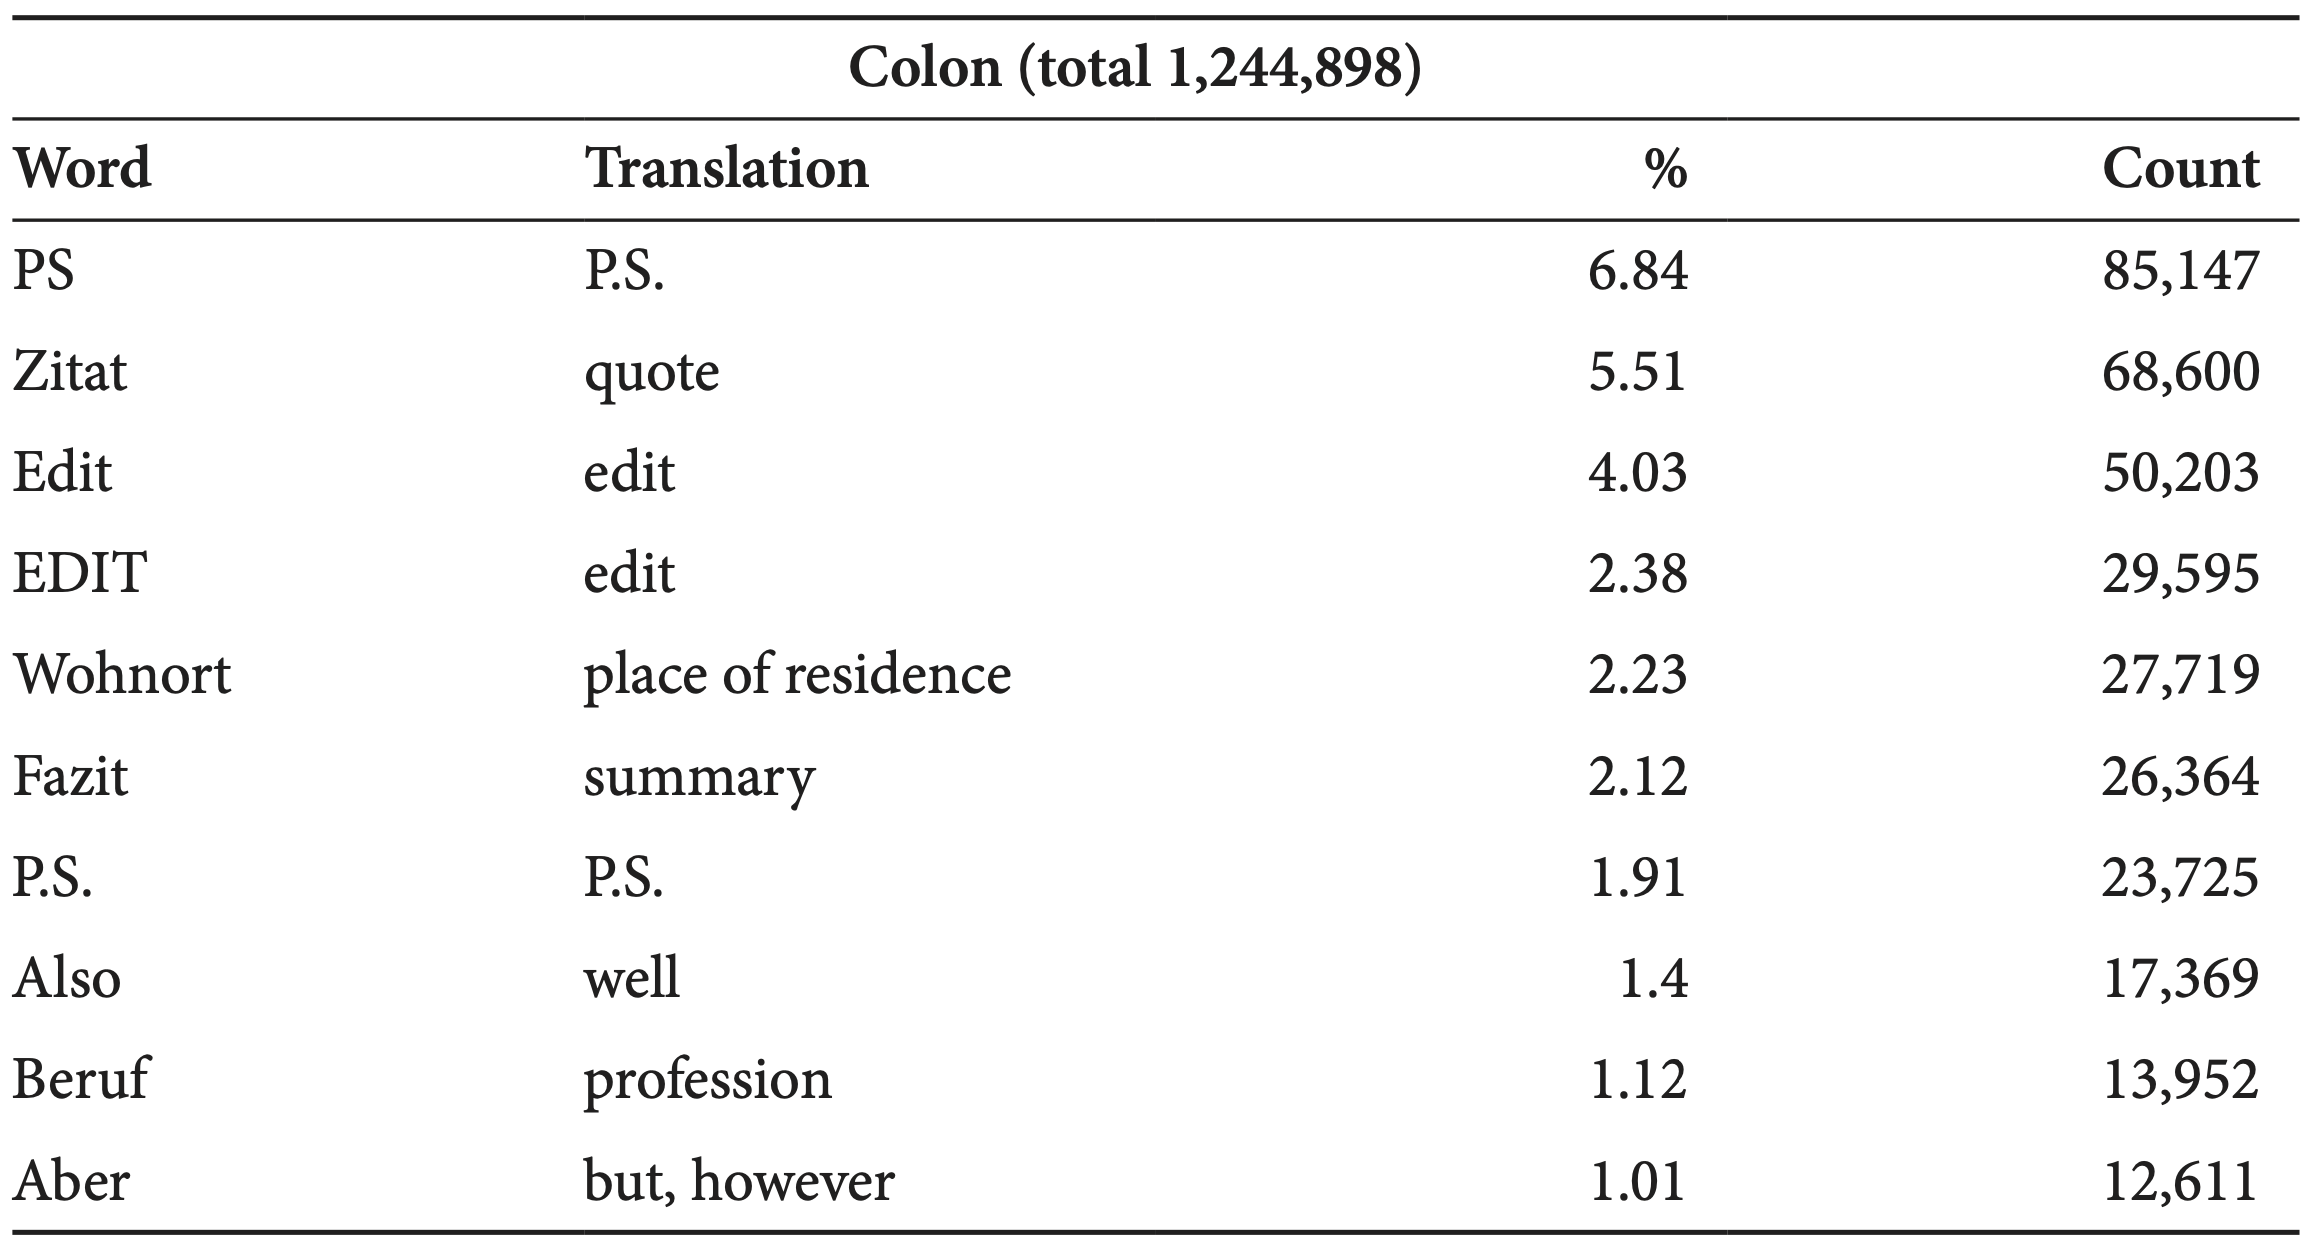
\includegraphics[width=0.7\textwidth]{\GRAPHPATH/obweil/05-colon}
\end{frame}

\begin{frame}
  {Empirischer Befund II/2 | Wortverteilung bei Komma}
  \centering 
  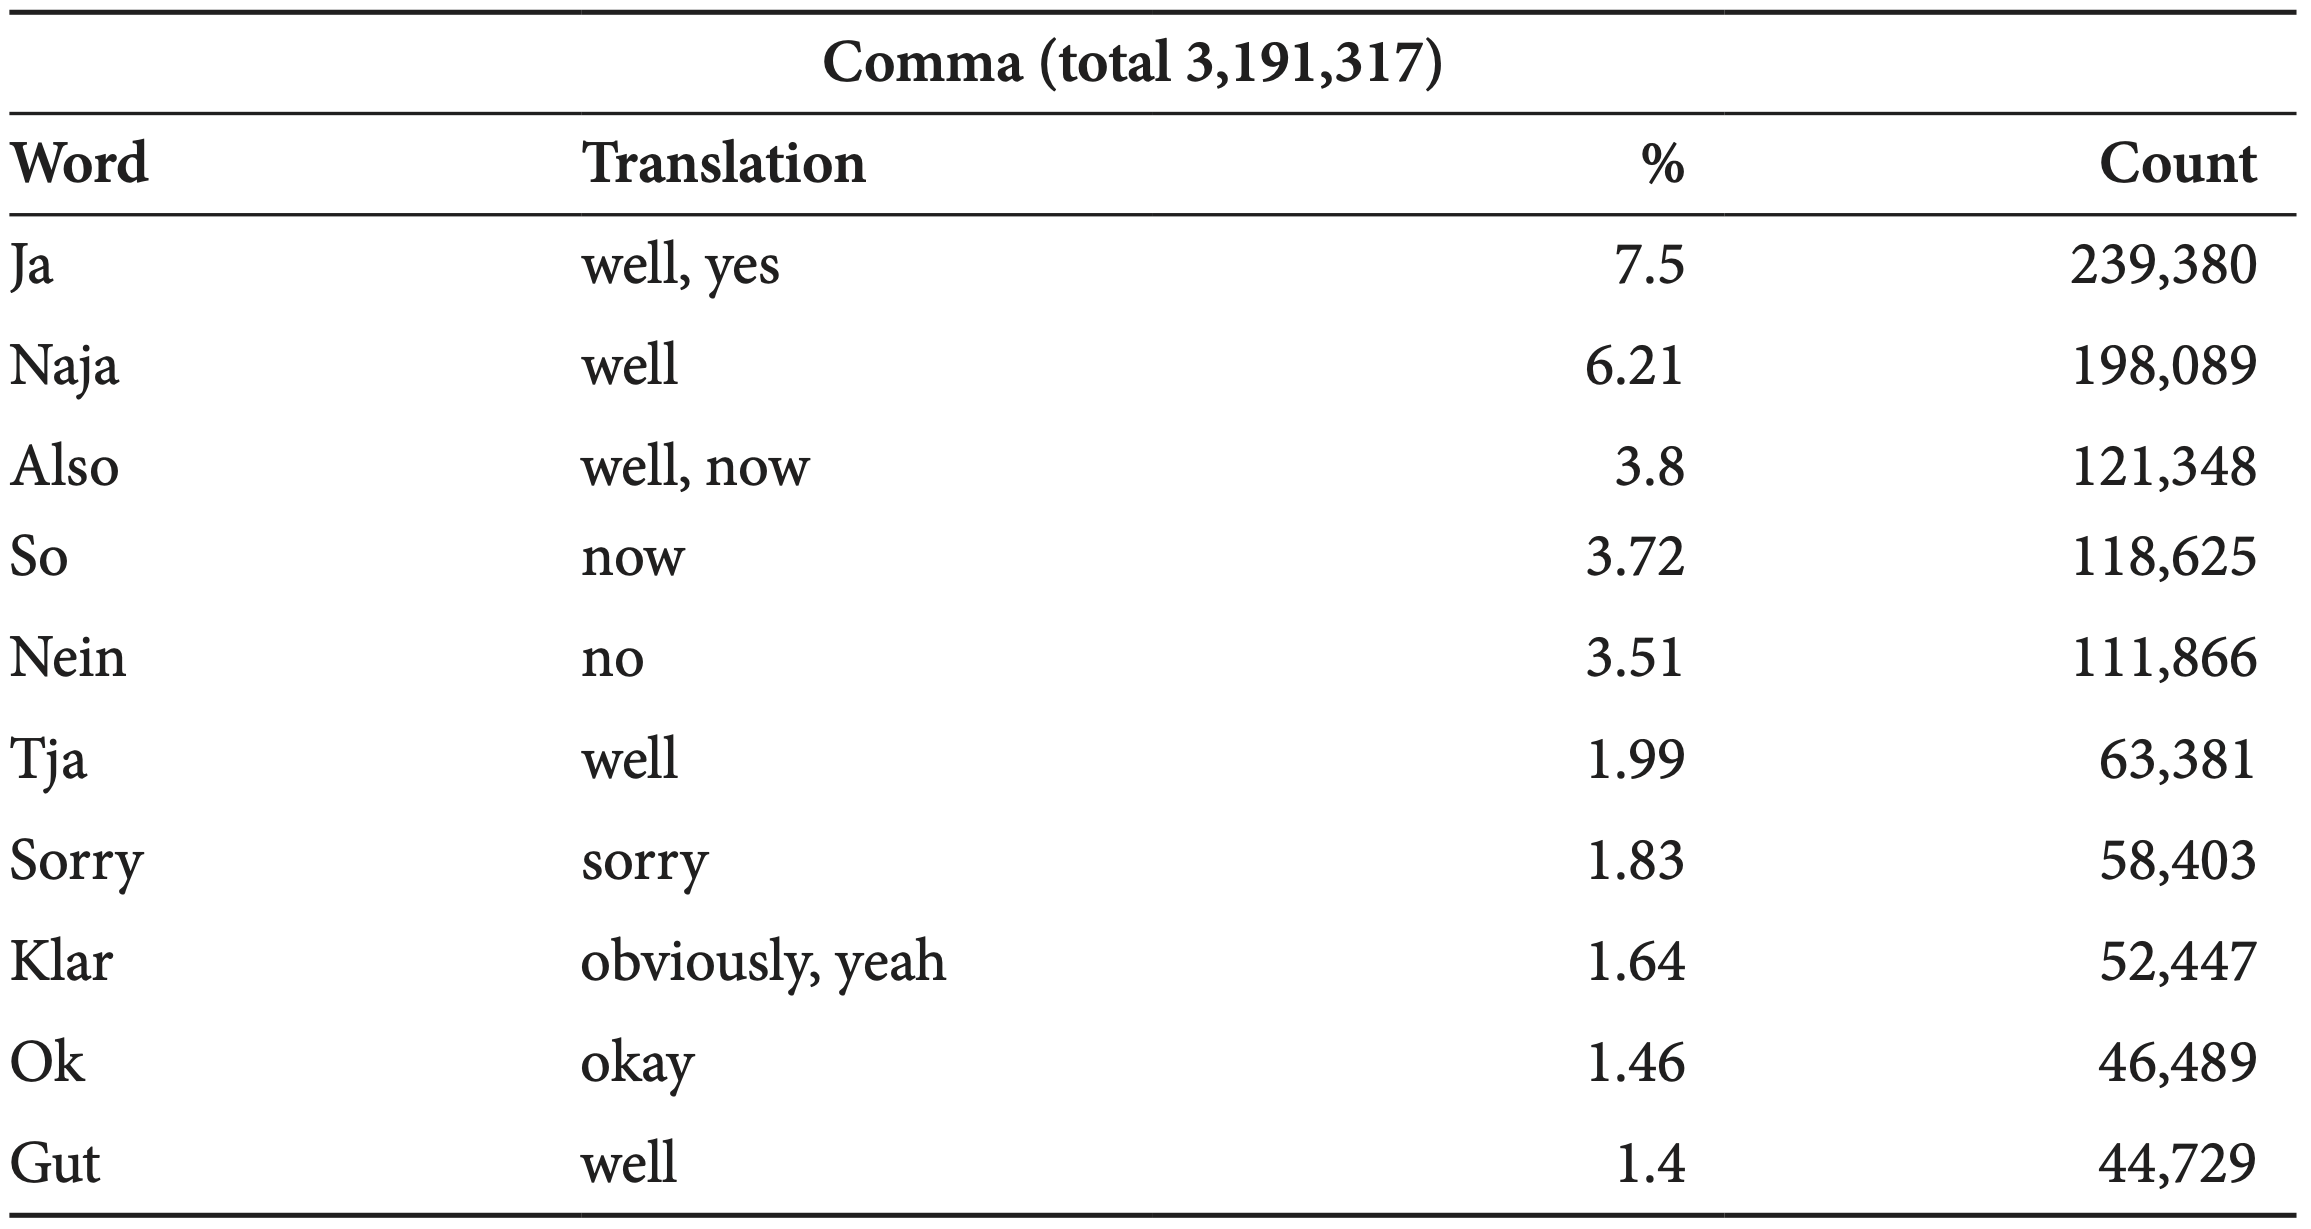
\includegraphics[width=0.7\textwidth]{\GRAPHPATH/obweil/05-comma}
\end{frame}

\begin{frame}
  {Empirischer Befund II/3 | Wortverteilung bei Bindestrich}
  \centering 
  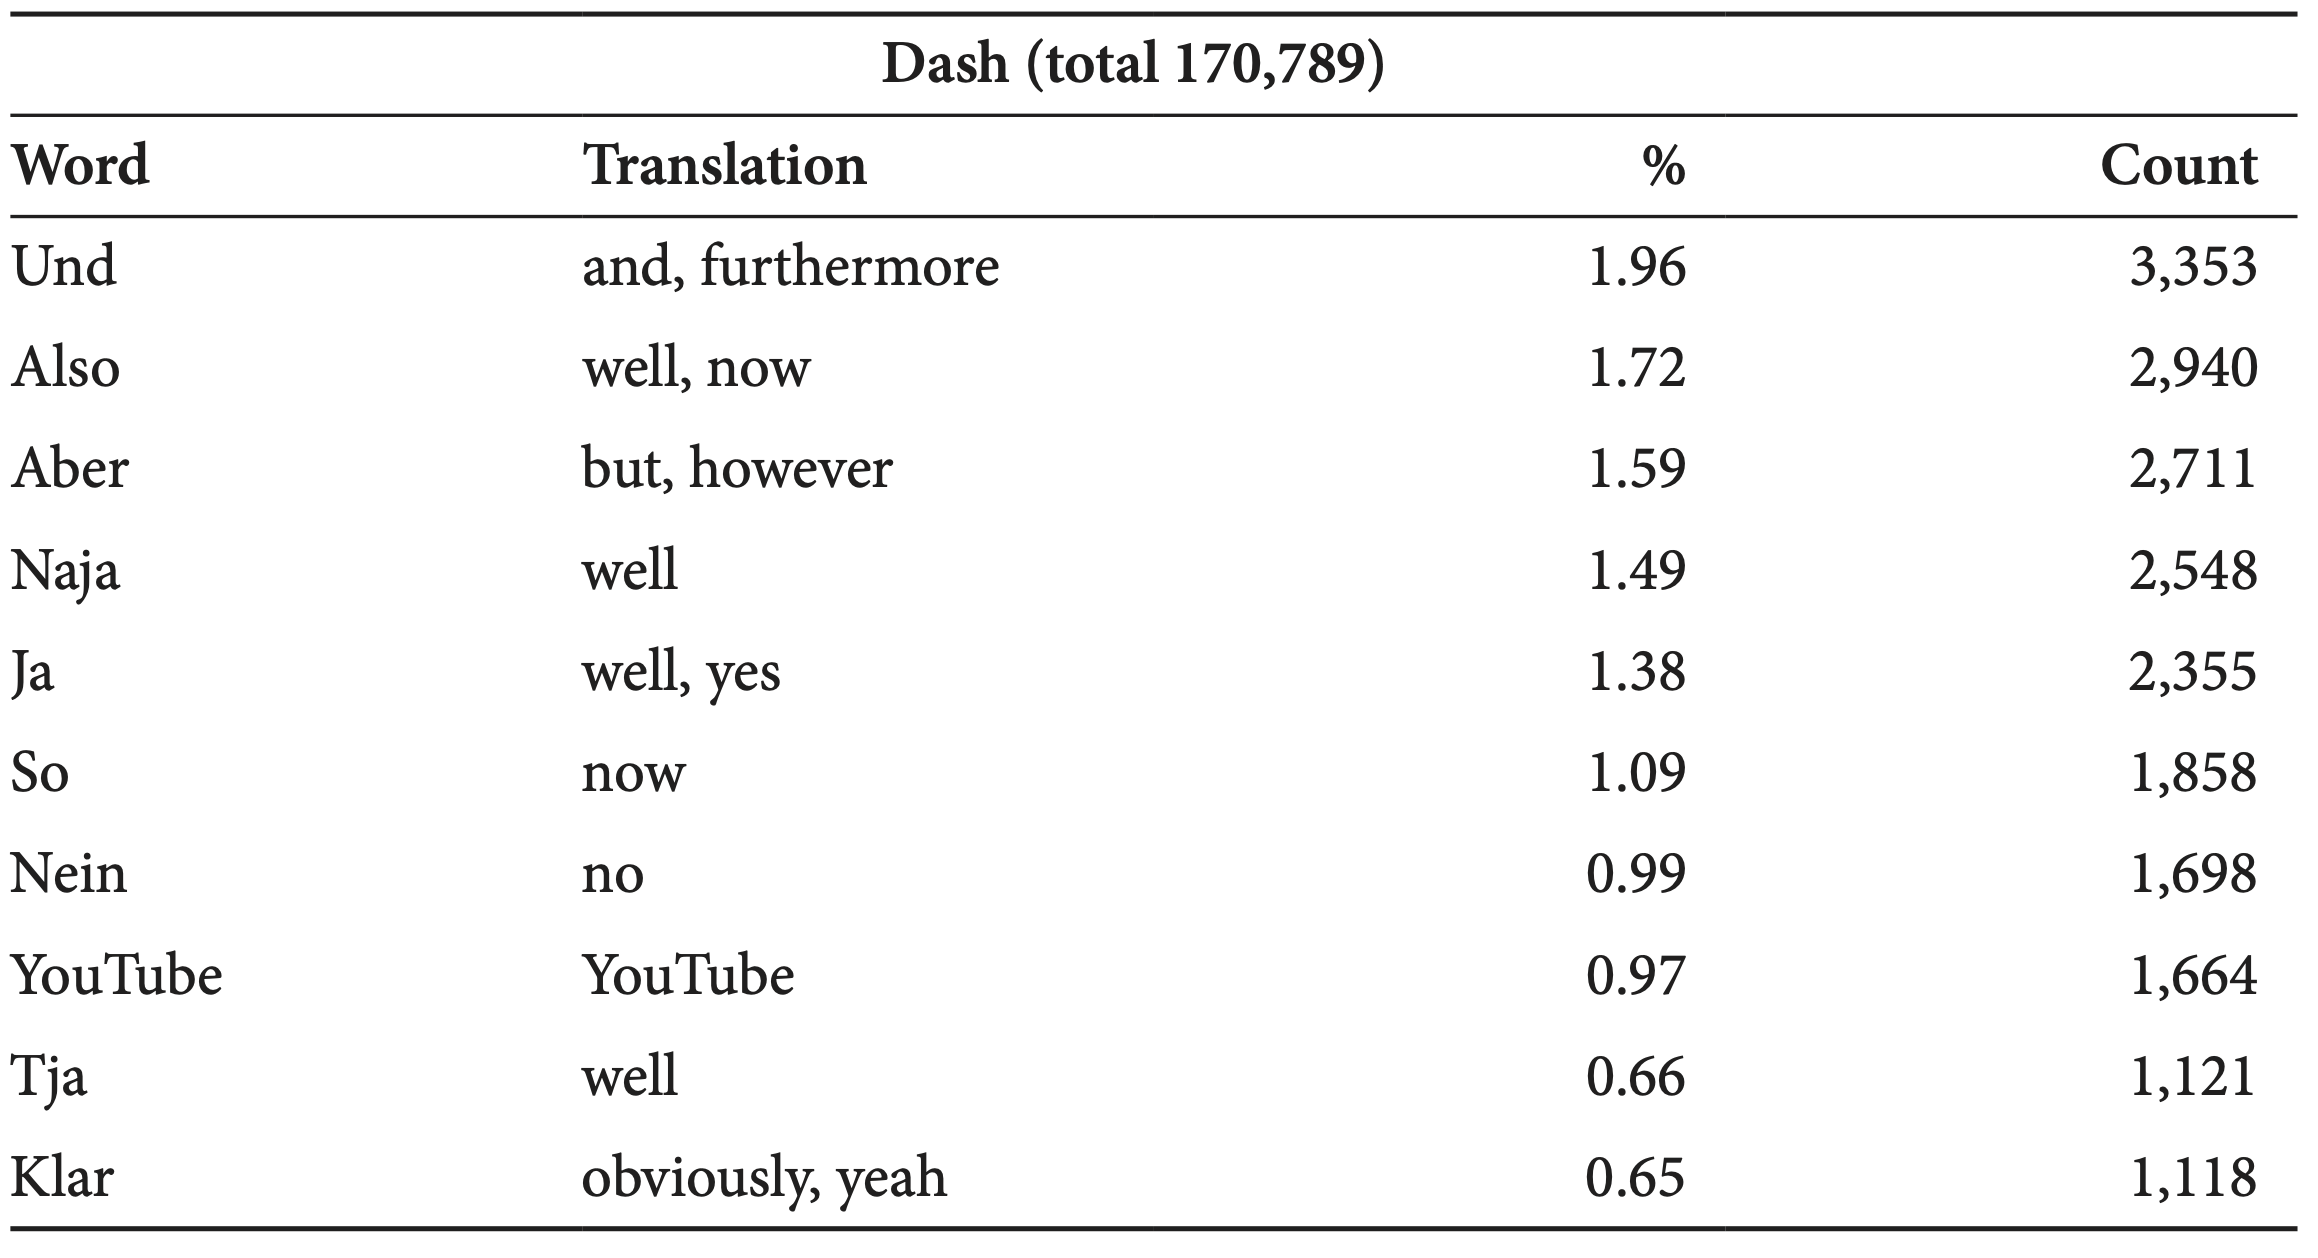
\includegraphics[width=0.7\textwidth]{\GRAPHPATH/obweil/05-dash}
\end{frame}

\begin{frame}
  {Empirischer Befund II/4 | Wortverteilung bei Dreipunkt}
  \centering 
  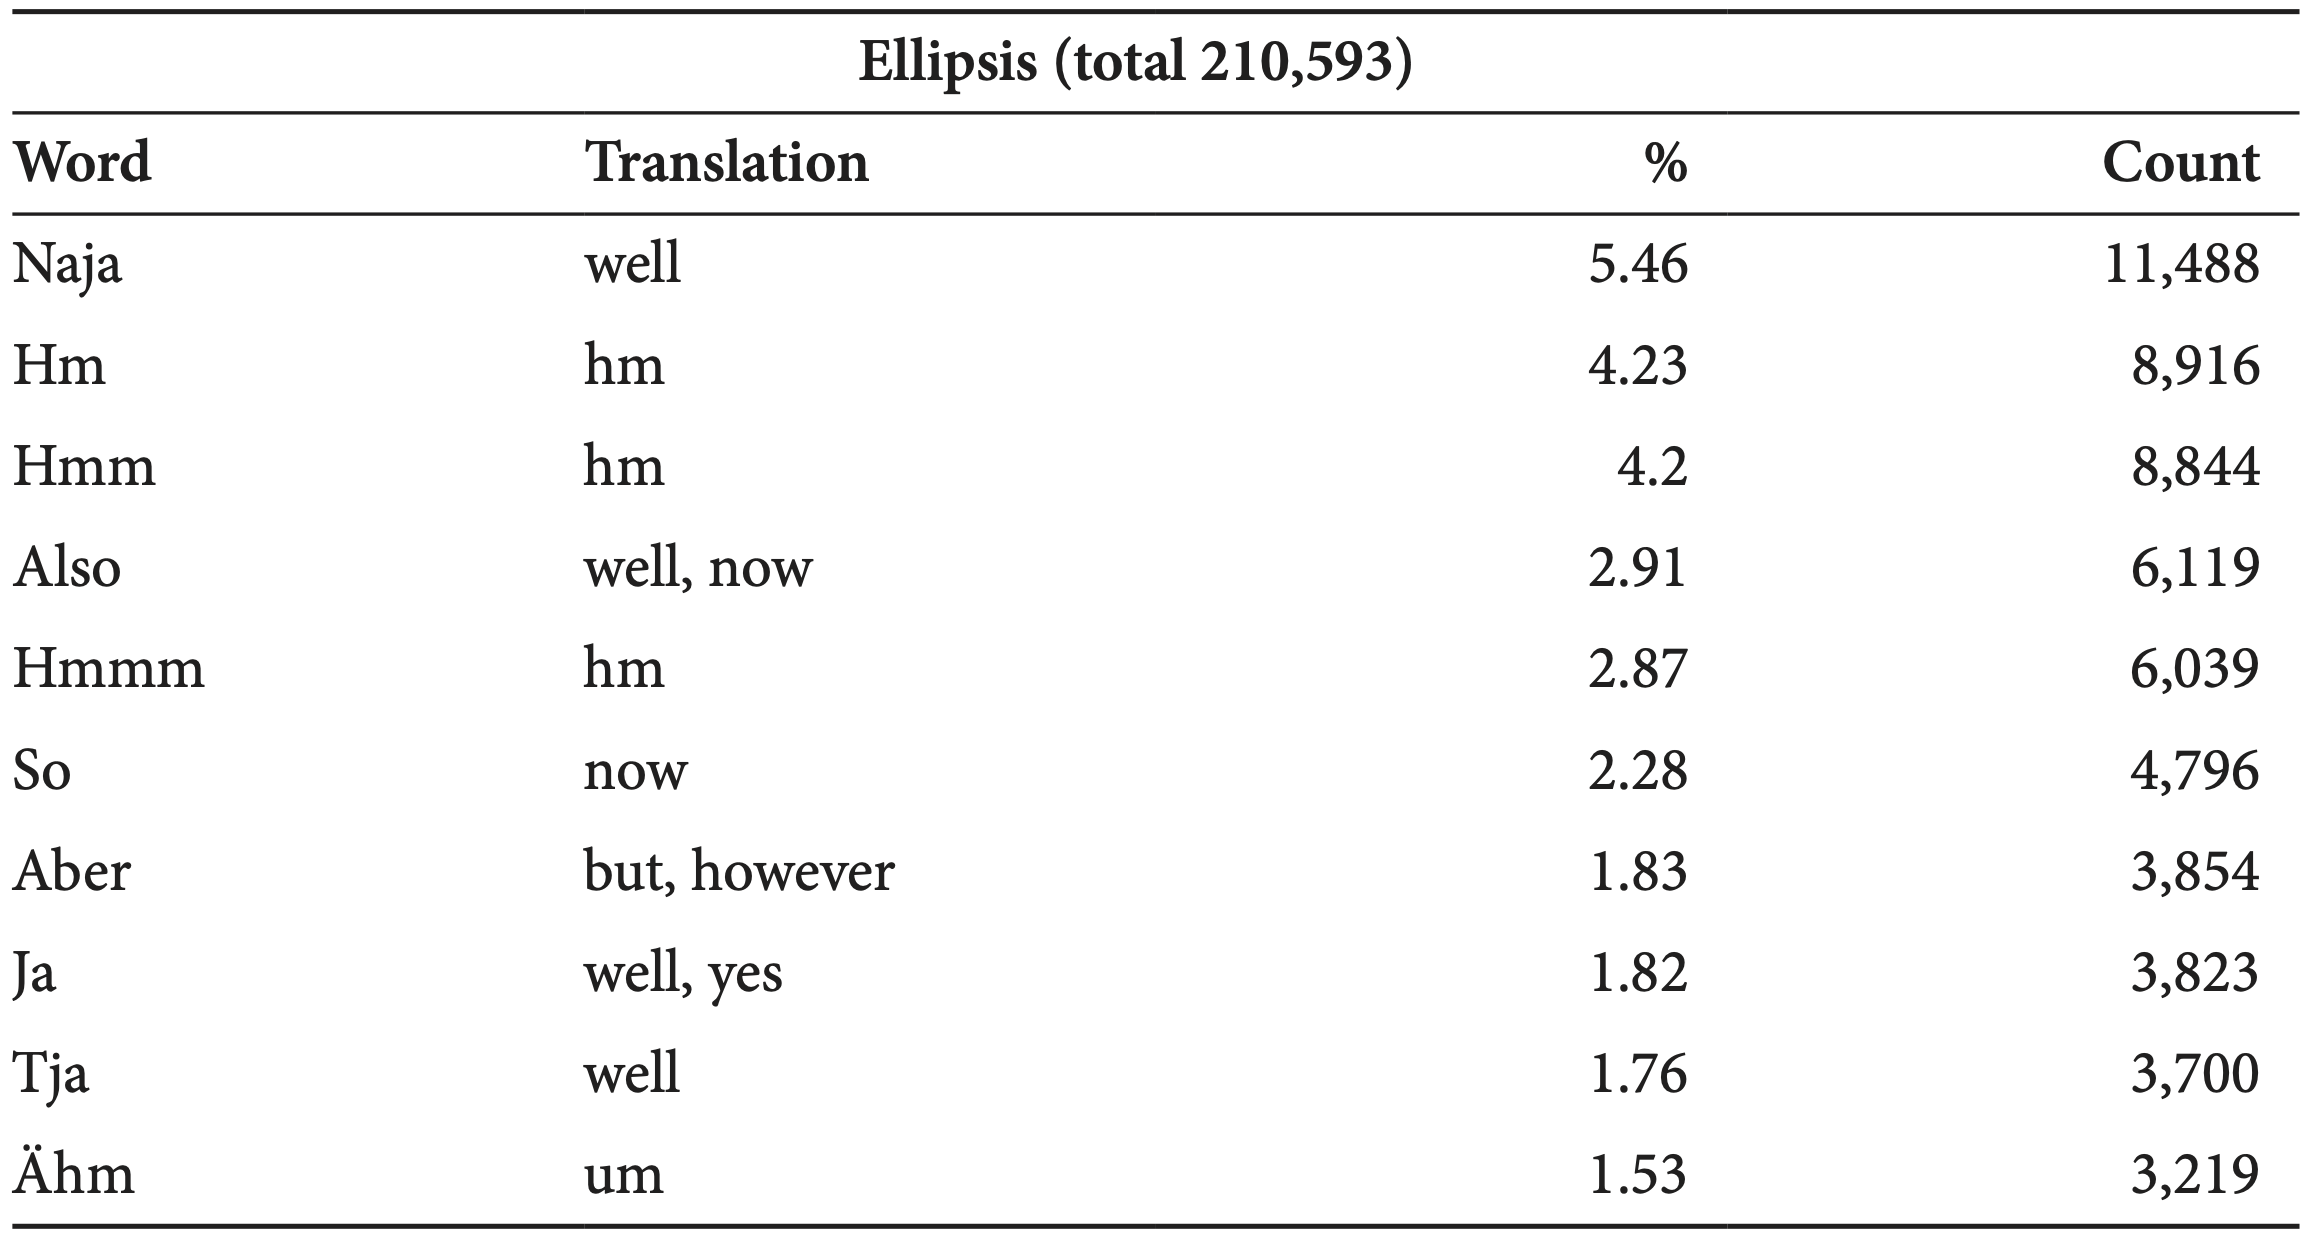
\includegraphics[width=0.7\textwidth]{\GRAPHPATH/obweil/05-ellipsis}
\end{frame}

\begin{frame}
  {Empirischer Befund III/1 | Links von \textit{obwohl}\slash \textit{weil}}
  \centering 
  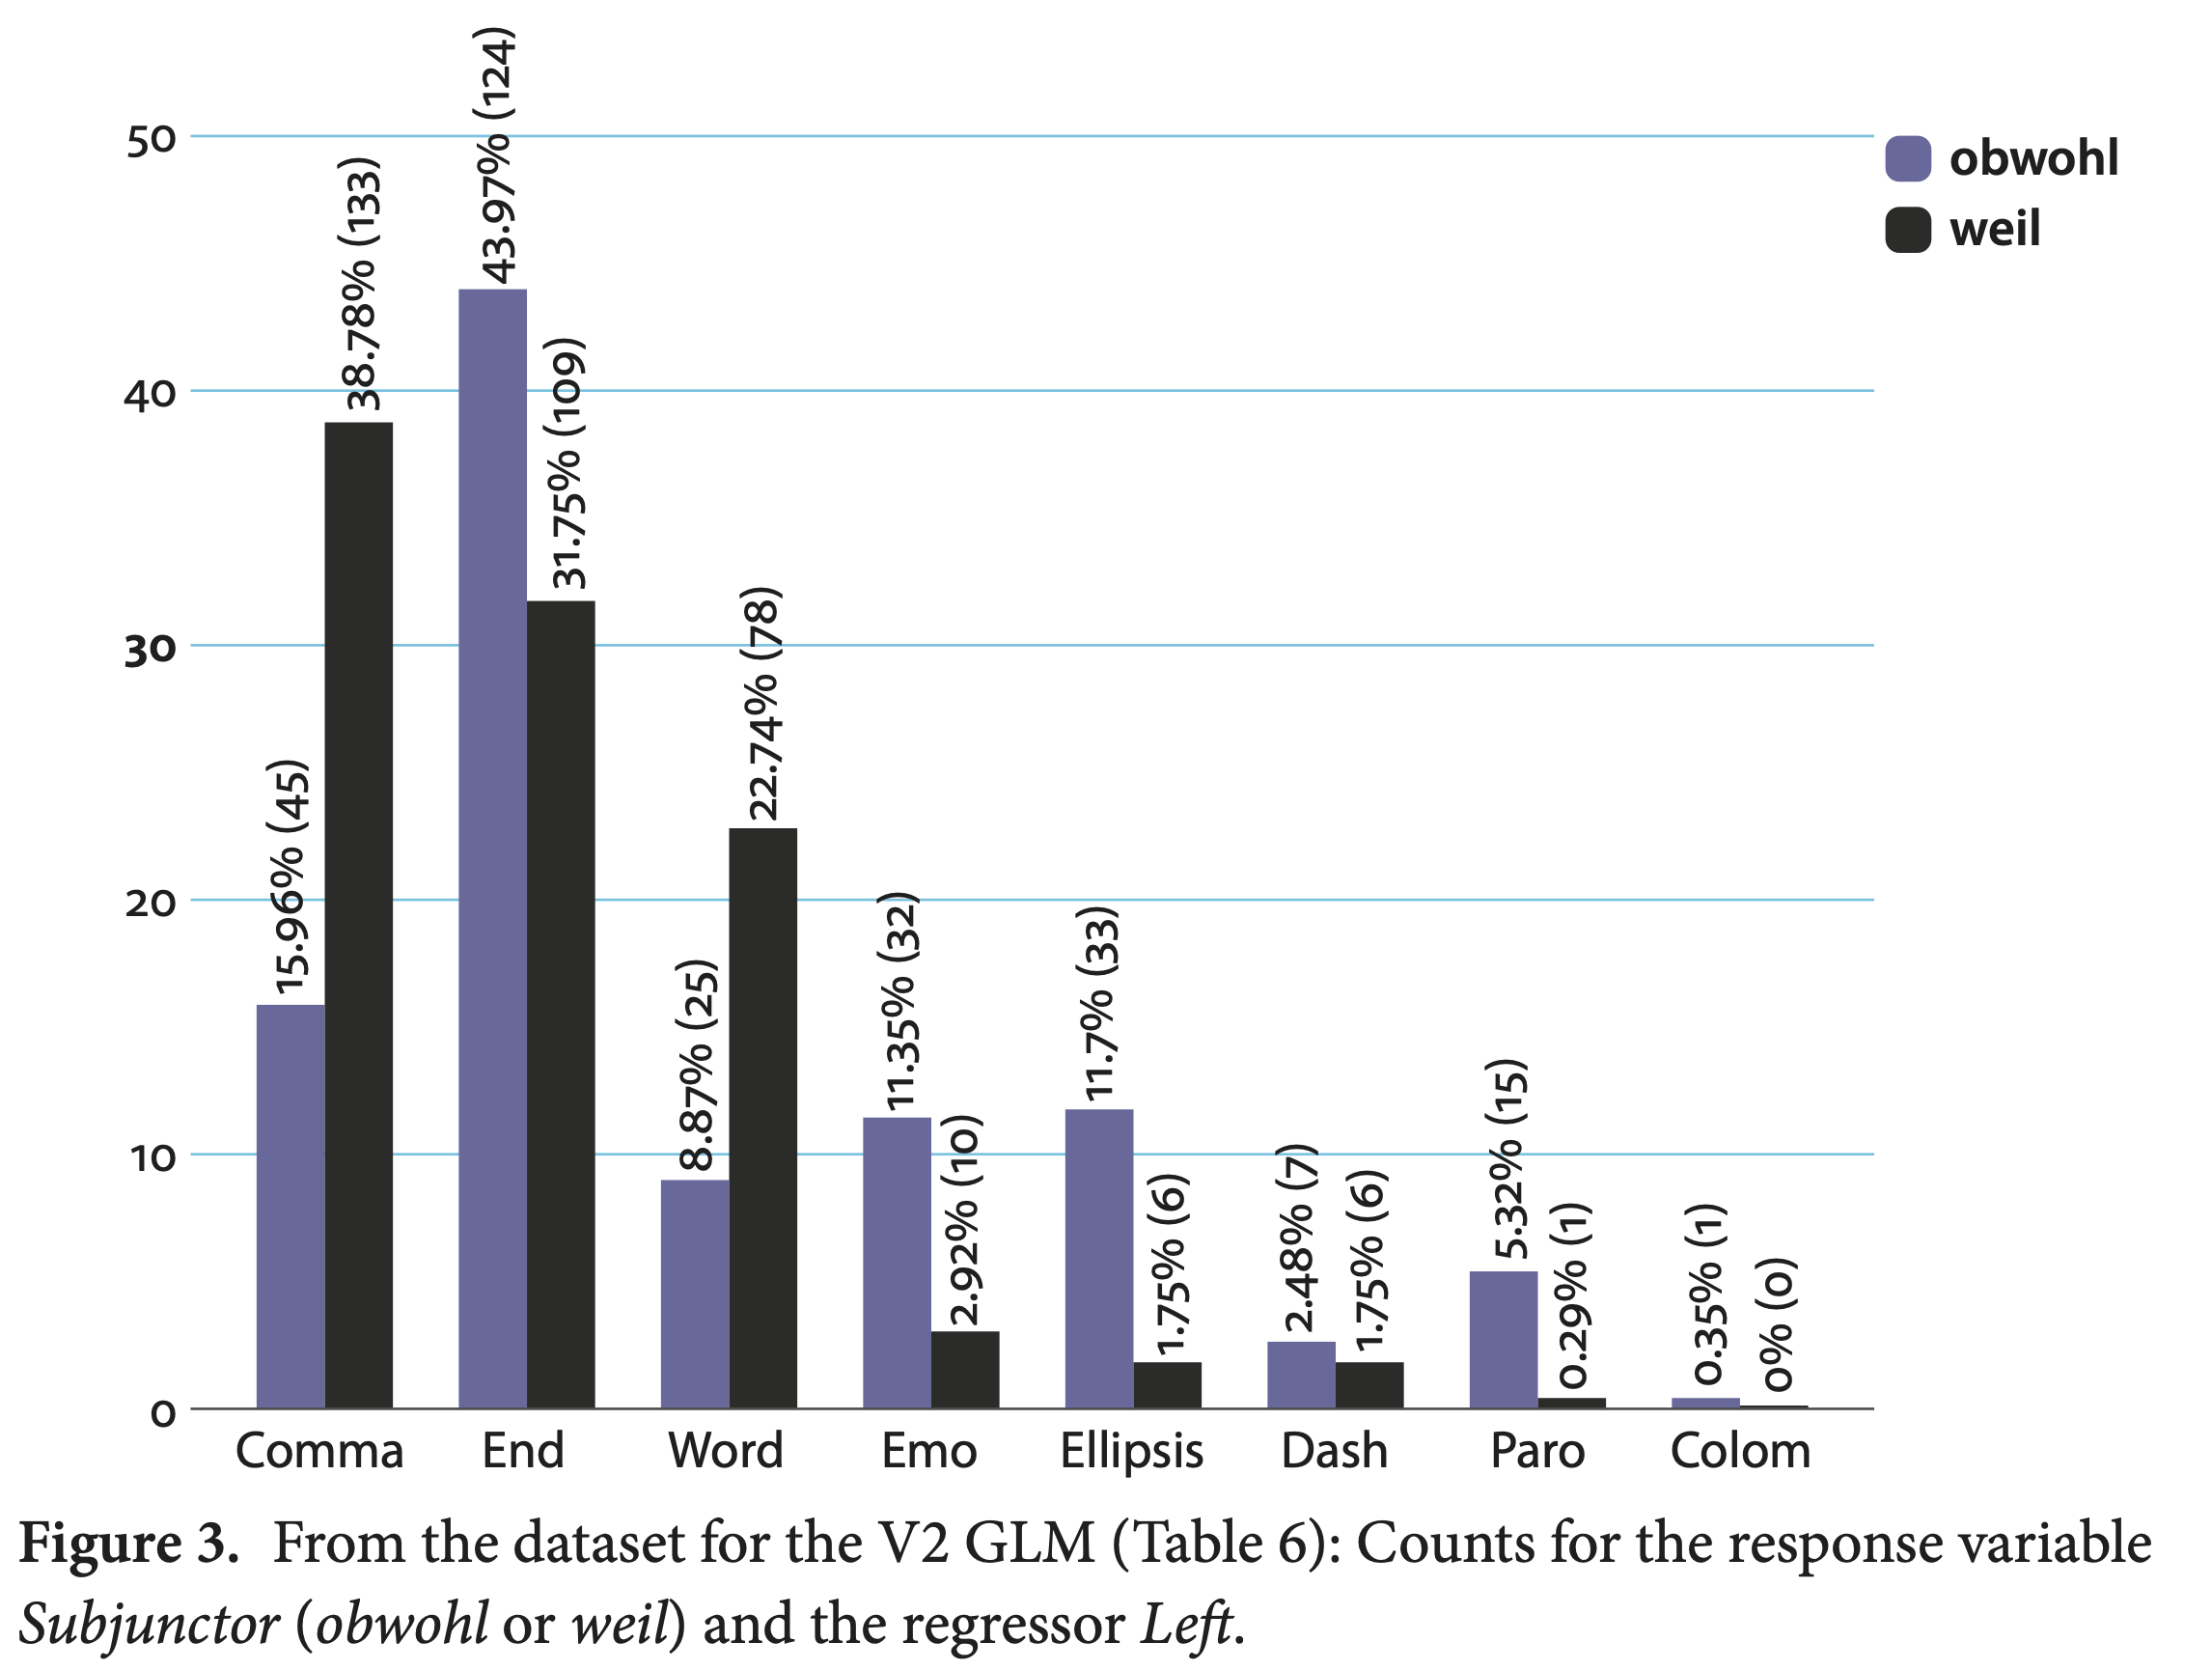
\includegraphics[width=0.7\textwidth]{\GRAPHPATH/obweil/06-left}
\end{frame}

\begin{frame}
  {Empirischer Befund III/2 | Rechts von \textit{obwohl}\slash \textit{weil}}
  \centering 
  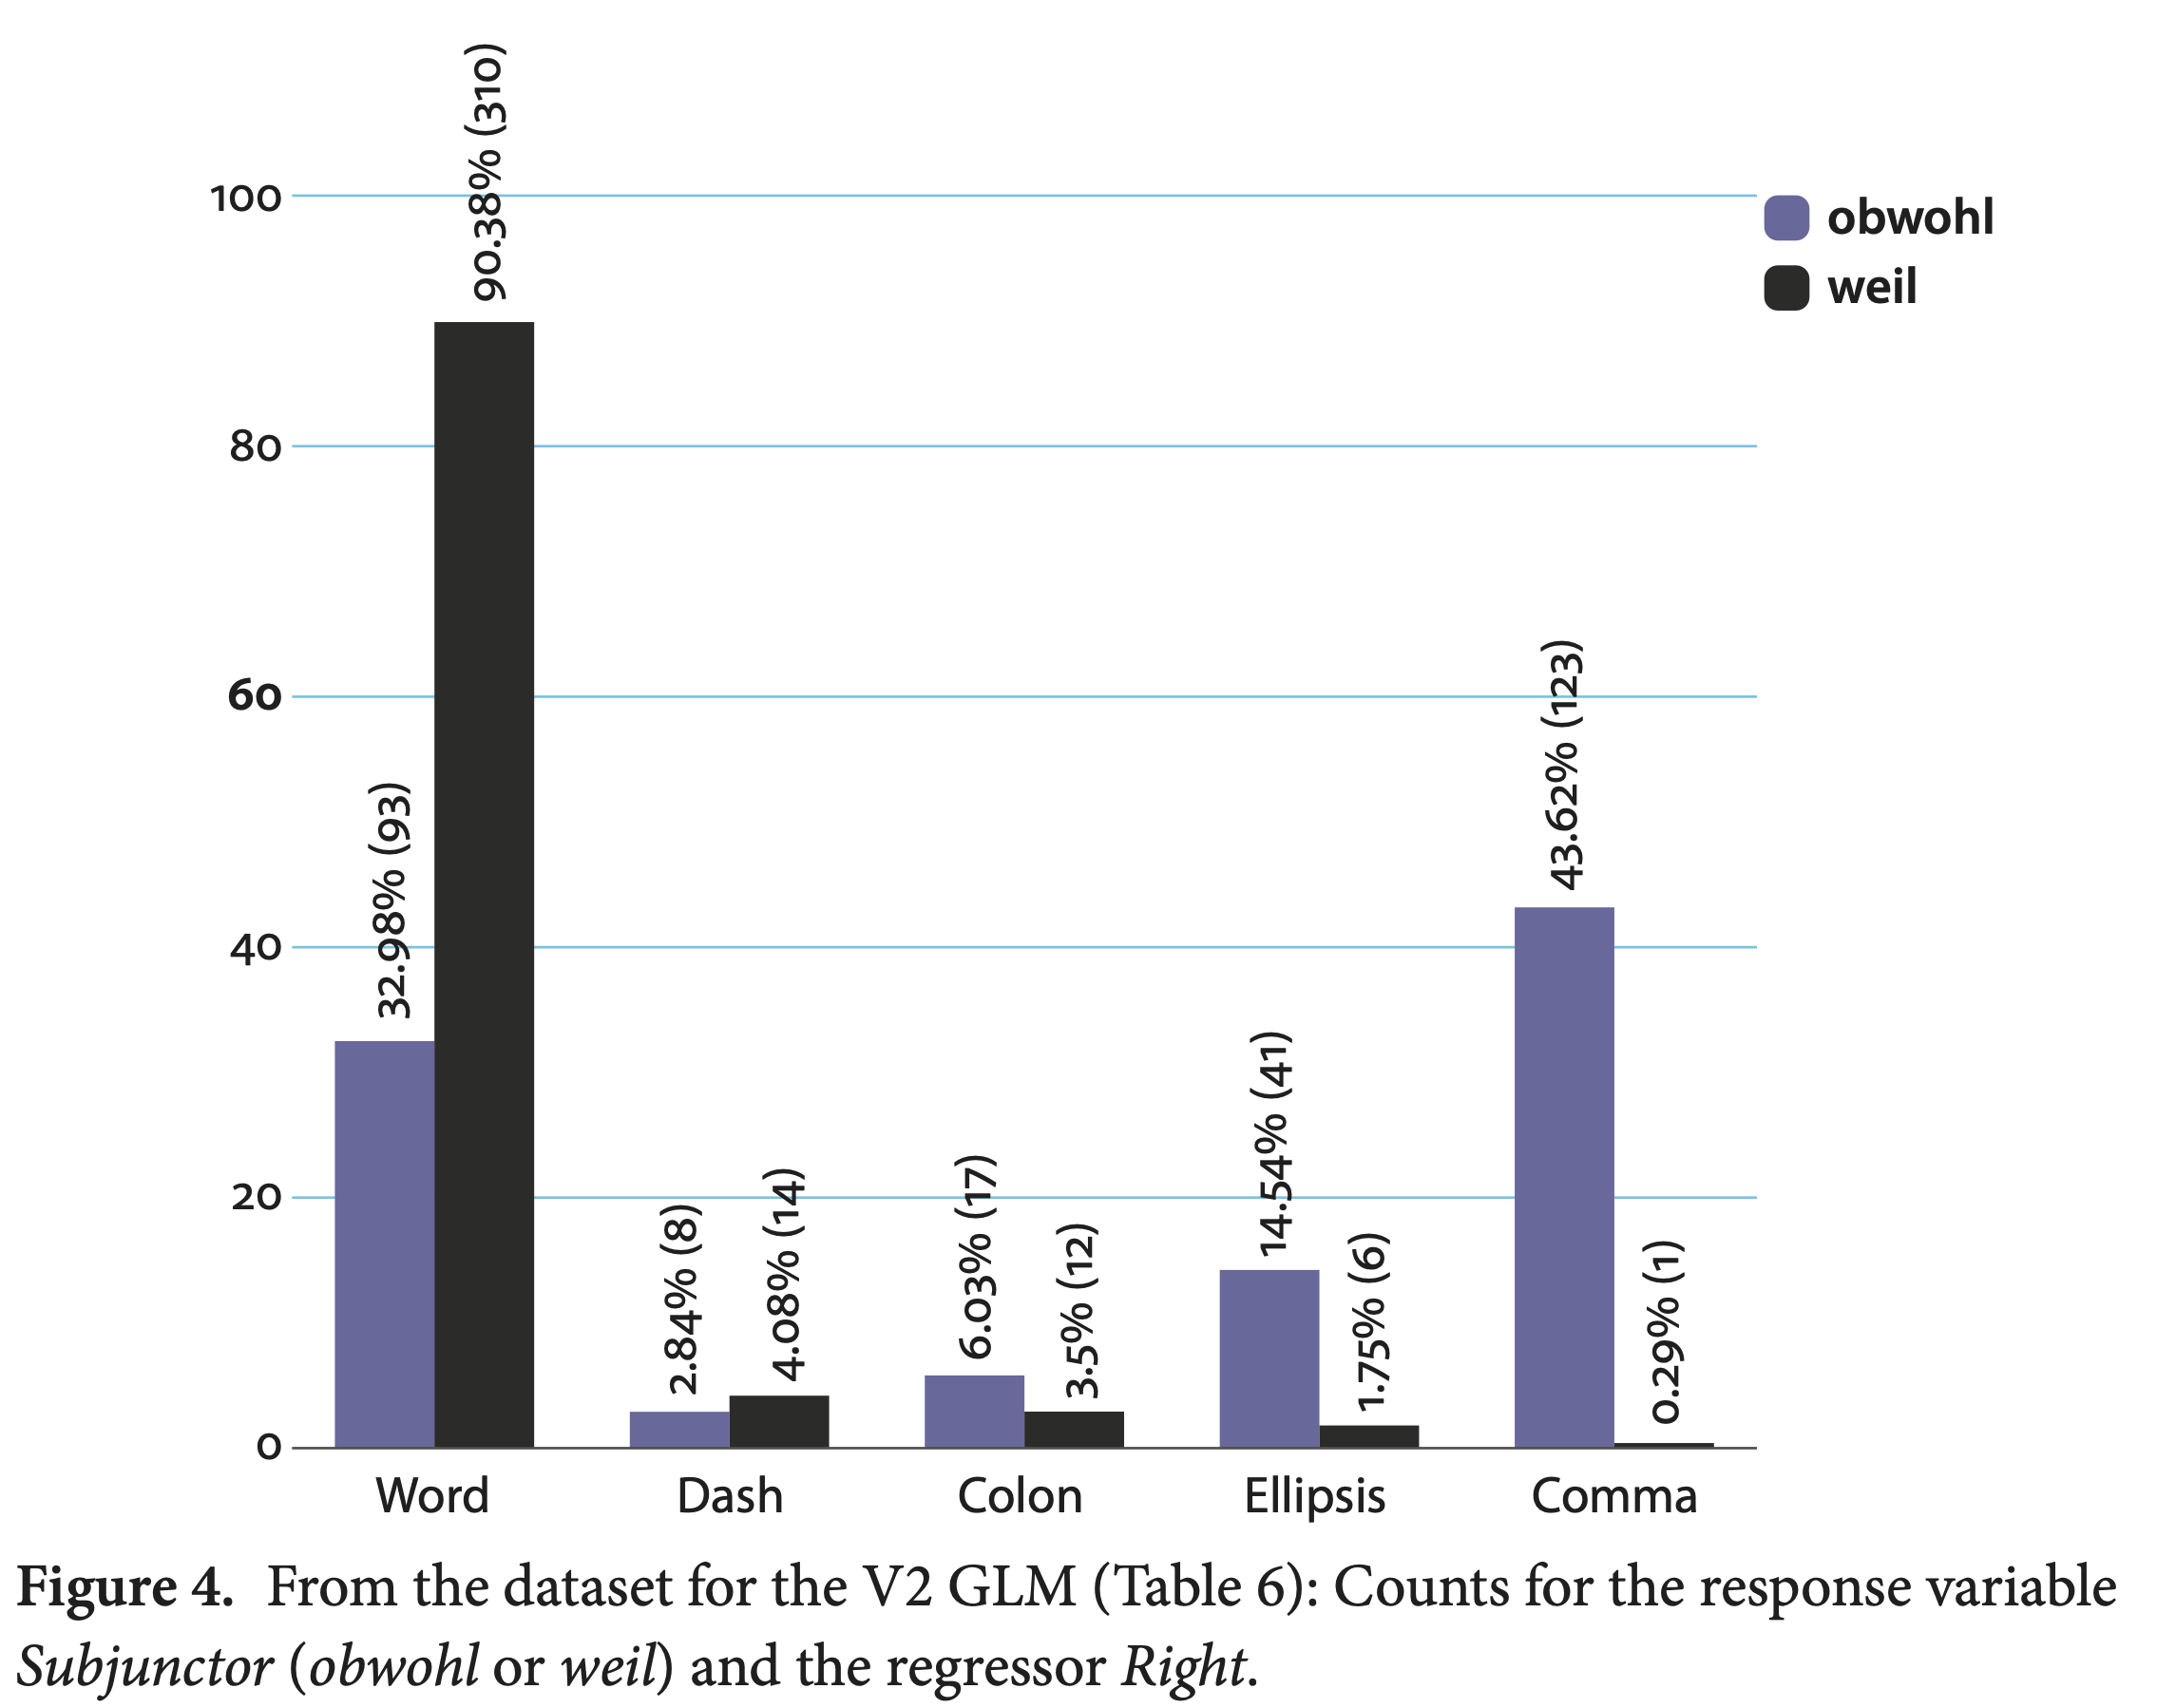
\includegraphics[width=0.7\textwidth]{\GRAPHPATH/obweil/06-right}
\end{frame}

%\section{Ausblick}


